\documentclass[11pt,twoside,bibtotoc]{scrartcl}
%\documentclass[12pt, a4paper]{article}

\newif\ifpdf
\ifx\pdfoutput\undefined
\pdffalse % we are not running PDFLaTeX
\else
\pdfoutput=1 % we are running PDFLaTeX
\pdftrue
\fi

\ifpdf
\usepackage[pdftex]{graphicx}
\else
\usepackage{graphicx}
\fi

\usepackage[utf8]{inputenc}
\usepackage[english]{babel}
%\usepackage{german}
%\usepackage{longtable}
%\usepackage{tocbibind}
%\usepackage{makeidx}
\usepackage[pdftex,pageanchor,colorlinks,pdfborder=0,breaklinks,urlcolor=blue]{hyperref}
\usepackage{amsmath}
\usepackage{amsfonts}
\usepackage{amssymb}
%\usepackage{pdfsync}  % enable tex source and pdf output syncronicity
%\usepackage[all]{xy}
\usepackage{multicol}
%\usepackage{rotating}
%\usepackage{wrapfig}
%\usepackage{subfigure}
%\usepackage{listings}

\usepackage{geometry} % to change the page dimensions
\geometry{a4paper}
\geometry{textwidth=16.0cm,textheight=24.5cm}
\geometry{left=3.0cm,twoside}
\parskip=0 cm
\parindent=0.0cm

\renewcommand{\baselinestretch}{1.2}

\newcommand{\mytitle}{Tool support for user testing of stereoscopic fatigue}

\usepackage{fancyhdr} % This should be set AFTER setting up the page geometry
\pagestyle{fancy} % options: empty , plain , fancy
\fancyfoot{}
\fancyfoot[LE,RO]{\textrm{\thepage}}
\fancyfoot[LO,RE]{\textit{Roethlin, G. 2008}}

\renewcommand{\labelitemi}{-}

\newcommand{\todo}[1]{{\LARGE TODO: #1}}

% Depth of the TOC
%\setcounter{secnumdepth}{3}
%\setcounter{tocdepth}{2}

\hypersetup{
    pdftitle={\mytitle},
%    pdfsubject={Subject of the document}, % Subject 
    pdfauthor={Gerhard Roethlin},              % Author
    pdfkeywords={master, fatigue testing software, stereo vision},       % Keywords
}

\title{Master Thesis: \mytitle\\
{\large Designing and implementing a flexible and extensible testing framework}}
\author{\normalsize Gerhard R\"othlin 
{\texttt{\href{mailto:cbreak@the-color-black.net}{cbreak@the-color-black.net}}}}
\date{2008.01.07 - 2008.07.07}

\ifpdf
\DeclareGraphicsExtensions{.pdf, .jpg, .tif}
\else
\DeclareGraphicsExtensions{.eps, .jpg}
\fi

\begin{document}

\maketitle

\begin{center}
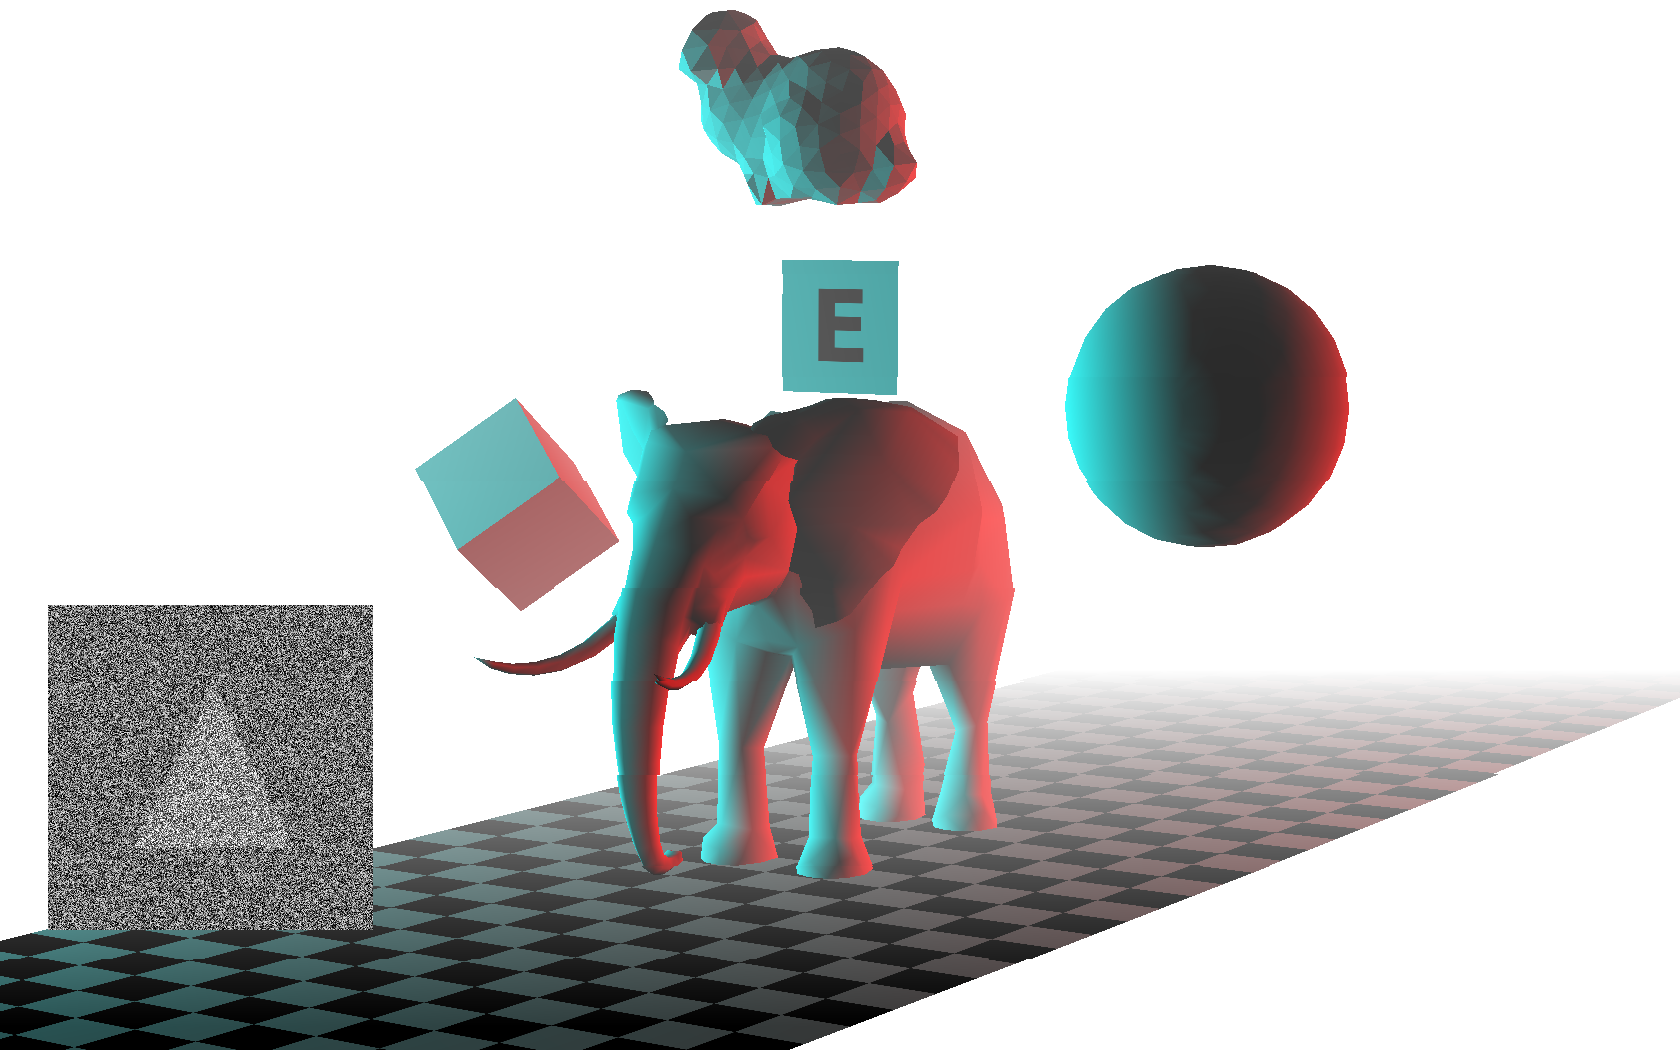
\includegraphics[width=15cm,clip,trim=0cm 0cm 0cm 0cm]{media/title.png}
\end{center}

\begin{multicols}{2}

\section{Abstract}
\paragraph{}
 \begin{abstract}
Viewing stereoscopic movies or images is unnatural. The focus and vergence of the eyes have to be decoupled. This strains the eyes, and can lead to fatigue, which makes the consumption of stereoscopic information over longer periods of times hard. But what are the physiological and psychological limits of stereoscopic viewing fatigue? And how can stereo images be composed to reduce fatigue?

Topic of this thesis is to write a Tool that enables exploration of those and similar other questions by providing a flexible and extensible framework for user testing. It is currently unclear how fatigue can be measured properly, and what scenes can be used to specifically test fatigue. Finding out which methods work and which do not is also part of this thesis.
\end{abstract}
\section{Design\label{Design}}
\paragraph{}
Implementing a flexible and powerful framework for user testing of stereoscopic problems requires a design that accounts for some special requirements. To find out what those requirements are, several tests where designed and executed. The design of the application was adapted to be fit for use in those and many other imaginable tests.

\paragraph{Creation}
The framework is split into three parts: The test design part aids with the construction of the test scene. A scene is a description of stimuli, possible inputs, and reactions to them. Traditional tests in this area show a series of pictures, requiring user feedback for each, while measuring the response time and the correctness. Stimuli are often precomputed and only consist of a single pixel image.

The requirements for stereoscopic test are different: It is not feasible to manually prepare stimuli, especially if complexe interaction is required. A method to generate them on the fly is needed.
Section \ref{sceneRep} describes how the look of a scene could be represented.

\paragraph{Testing}
The testing part is the most important. It displays stimuli and logs the user replies, reacting in a way that is defined by the designer of the test. While traditional tests only follow the question-response pattern, stereoscopic user tests often require more: Trials often have to be randomized with several constraints, simply randomizing might lead to overlaps, or imbalances in dependent properties. All parameters of the stimulus have to be directly or indirectly controllable based on user input such as movement of stimuli, movement of the camera, or visibility of objects.

\paragraph{Analysis}
Analysing the gathered data is the third part. This is usually done in a combinataion of Microsoft\texttrademark\ Excel\texttrademark\ and highly specialized data analysation methods such as Anova. Both are sophisticated and well known by the users.

The easiest way to achieve compatibility with the known procedures is to produce data in a format, that is evaluatable in those tools. A log transformation program can take care of this in most tests: The time stamp based logs get parsed, and challenge-response times get measured and written in a format importable by spread sheet applications.

Some tests might not follow this pattern, and the data has to be analysed in a different way.


\subsection{Representation of a Scene\label{sceneRep}}
\paragraph{}
Scene graphs are used to store scenes in a structured way. They have been continually developed since their invention\cite{scenegraph} to account for spatial, state, hierarchy and other properties. Many scene graph libraries exist, but they are usually focused on a specific field, and part of a bigger framework.

To be able to control inconsistencies such as individual depth cues, it is required that the scene graph can represent these. Nodes could add or remove cues for their children, giving a maximum of control to the users. Scene graph libraries do not support those requirements. Designing a simple scene graph is required.

\subsubsection{Node types}
\paragraph{}
Scene graphs are tree structures consisting of nodes with zero or more child nodes. The scene itself is typically the root node, while actual rendered objects often are leaves. The following nodes are planed to be implemented in the framework.

\begin{description}
\item[Rectangle] A primitive geometry node, which has the shape of a parallelogram. The node can reference a texture, which gets mapped on it's surface.
\item[Parallelepiped] A primitive geometry node, which has the shape of a parallelepiped (parallelogram prism). As it's parent it can be textured.
\item[Pixelplane] A primitive geometry node. It is used to draw pixel exact images at any position in space. It requires a texture to be visible. Pixelplanes are point shaped, and therefore are not influenced by scaling and rotation.
\item[Text] A primitive geometry node. It draws text at any position in space, similar to Pixelplanes.
\item[Mesh] A primitive geometry node who's geometry is defined by a mesh. The mesh can contain vertex normals and vertex texture coordinates. A texture can be mapped on the object. It might be desirable to also include vertex color.
\item[AffineTransformation] A group  node. It contains other nodes, which it can affine transform by directly manipulating the matrix stack.
\item[Camera] A group node. It contains other nodes, which are rendered by this camera instead of the global camera. This is used to control projection cues in a consistent way. Has to reset the depth buffer.
\item[DepthBuffer] A group node. Disables or enables the use of the depth buffer for all contained elements. This is used to disable occlusion clues. Can reset the depth buffer.
\item[Lighting] A group node. Enables lighting and a light source with controllable parameters for all sub nodes. This is used to enable lighting depth cues.
\item[Atmosphere] A group node. Enables the fog equation and controls its parameters. This is used to enable aerial depth cues.
\end{description}

\paragraph{}
The following nodes are problematic and might be hard to use, implement and understand due to their side effects.

\begin{description}
\item[XSize] A group node that scales objects to add or remove depth cues caused by perspective projection. It can be implemented on object (scale object individually, without consider intra object depth) or space level (scale  as function of depth, which is similar to a camera projection). Either way has it's own problems.
\item[XOffsest] A group node that moves objects it contains as function of their camera distance. Can be used to add or remove height-of-field, convergence or motion parallax cues.
\end{description}

\subsubsection{Node organisation}
\paragraph{}
\todo{Write about simple trees, parallel scene graphs, object soup}


\subsection{Mechanics of a Scene\label{sceneMech}}
\paragraph{}
\todo{Write about what makes a scene move, the code/interaction. Write about Procedual(LUA) and Finite-state-machine(Custom)}


\section{Cues\label{Cues}}
\paragraph{}
Seeing stereo is not only based on binocular stereopsis.There are several aspects of the visual impression that allow the perception of depth. Common depth cues include accommodation, aerial perspective, binocular disparity, convergence, height in visual field, motion perspective, occlusion, relative size, and relative density. In addition others have been suggested, such as linear perspective, light and shading and texture gradients.%, kinetic depth, kinetic occlusion and disocclusion, and gravity.

Cutting and Vishton\cite{DepthCues} analyzed nine of these depth cues to asses their relative strength. Those cues will be described in the following paragraphs, and their reproduction or elimination on screen in a digitally generated scene is discussed. The use of OpenGL or a similar technology is assumed, techniques like ray-tracing or vector based painting may require different methods.


\subsection{Projection based cues}
\paragraph{}
These cues are caused by the way the 3D world gets projected onto the 2D surface of the retina.
Even though the reason that each of them exists is the same, the way they are evaluated and their reproduction is different.

Most projections\cite{proj} that are in use, map a ray in the world space onto a single point in the image space. Parallel Projection\cite{parallel} and Perspective Projection\cite{perspective} are the most commonly used methods. Physical optics use a projection similar to perspective projection.

Since all the following cues are generated by the same cause, enabling and disabling each is not possible in a consistent way. There are two basic ways to get individual control anyway: Use one projection method for all parts of the scene, but compensate to remove or add clues. Or use one projection method for every part of the scene, and compose the resulting image. Careless use of either method can cause conflicts such as pinning, rivalry, or the inability to fuse the image.


\subsubsection{Relative size}
\paragraph{Description}
The size of objects relative to each other is a strong clue for their distance, but it requires knowledge or assumptions about the size of an object. Due to the perspective projection, objects further away from a viewer take up less space in it's field-of-view. When seeing a human, it's distance can be estimated fairly accurately.

Seeing an unknown object requires comparisons with other objects in the scene. Upon seeing a number of cubes with different perceived sizes, and without prior knowledge of their size, one could assume similarity in size, and derive depth relations between them.

\paragraph{Reproduction}
Relative size only works when the perceived size of an object changes with it's distance. Using a perspective camera is an easy way to do this. When creating an artificial image, the size change can also be simulated by scaling objects based on their distance to the camera. In the case of OpenGL or most RayTracers, both parallel and perspective cameras are available.

\paragraph{Non-reproduction}
If the size of objects is not intended to change with their distance from the viewer, either choosing a parallel projection or compensating the projection based scaling by scaling the object size is needed.


\subsubsection{Relative density}
\paragraph{Description}
Relative density is closely related to relative size. It concerns the projected density of objects, which are distributed regularly. When such a group of objects change in depth, or take up different depth areas, their change in perceived density yield information about the depth change.

\paragraph{Reproduction}
If a perspective projection is used, relative density changes are calculated correctly. Introducing relative density clues into a scene that is rendered with a parallel projection requires non uniform scaling.

\paragraph{Non-reproduction}
Eliminating the relative depth cue from part of a scene that is parallel projected requires non uniform scaling of a group of objects. Both the position relative to each other, and the size relative to each other of the objects has to change.


\subsubsection{Height in visual field}
\paragraph{Description}


\paragraph{Reproduction}

\paragraph{Non-reproduction}


\subsubsection{Motion perspective}
\paragraph{Description}

\paragraph{Reproduction}

\paragraph{Non-reproduction}


\subsubsection{Convergence}
\paragraph{Description}

\paragraph{Reproduction}

\paragraph{Non-reproduction}


\subsubsection{Binocular disparity and stereopsis}
\paragraph{Description}

\paragraph{Reproduction}

\paragraph{Non-reproduction}



\subsection{Other cues}


\subsubsection{Occlusion}
\paragraph{Description}
Objects that are in front of other objects relative to the viewer are perceived to occlude the object behind. Even transparent or translucent objects often change the appearance of objects they occlude. This allows to infer depth ordering of objects. This clue is very strong, and it's range is the longest of all depth cues. It does however not allow to judge the distance between objects.

\paragraph{Reproduction}
Reproducing this depth clue digitally requires extra work, since most output media do not have a notion of depth. A traditional approach is the Painter's Algorithm\cite{painters}. Objects are ordered by depth and drawn from far to close. Ordering objects has performance implications, and is not always possible.
A newer method that does not require sorting is the Depth Buffer\cite{zbuffer} (also known as Z-Buffer). For every pixel it's associated depth value is stored. New objects only replace pixels further away.

\paragraph{Non-reproduction}
Not reproducing this clue is fairly straight forward. Disabling the depth buffer allows ordering objects according to preferred depth appearance, independently of their actual depth coordinates. Objects that are both behind and in front of an other object have to be segmented into pieces. This is most commonly the case when objects intersect.

Objects that consist of several surfaces might require internal ordering to appear correct, which is expensive. One way to resolve this problem is to clear the depth buffer after every object drawing. Depending on the size of the image this might be costly also.


\subsubsection{Aerial perspective}
\paragraph{Description}
Areal perspective is related with Occlusion: Objects far away from the viewer are often occluded by the atmosphere, be it air, smoke, fog or water. Consequentially, objects far away change their appeared color, losing saturation, and chroma.
Unlike most depth cues, it gets more effective as the distance from the observer increases.

\paragraph{Reproduction}
Reproducing this cue requires extra work. A common approach is to mix the object color with a fog color, depending on it's distance to the observer. This is cheap, and can be enabled per object\cite{fog}. Weights of the mixing is determined by a fog equation.

\paragraph{Non-reproduction}
Not reproducing this clue is easy, and it is not enabled by default. Explicit control over the appeared depth can be achieved by individually changing the fog equation for each object.


\subsubsection{Accomodation}
\paragraph{Description}
Accommodation is the change in the shape of the lens of the eye, to keep the perceived image of the world sharp\cite{accommodation}. It is coupled with convergence. Viewing stereoscopic material requires that the accommodation stays the same, since all image information comes from a screen at a fixed depth.

\paragraph{Reproduction}
Artificially generating the requirement that the human eye changes accommodation is hard. It requires optics in between the eye and the screen, or the changing of distance to screen depending on the object that is focused. Neither is practical.

\paragraph{Non-reproduction}
Not reproducing this cue is almost required. Everything seen on a screen requires the same accommodation to be viewed as the screen itself. If a constant accommodation requirement throughout the scene exists, a screen at a huge distance, or a convex screen can be used.

\subsection{Stereogram\label{Stereogram}}
\paragraph{}
A stereogram is an image that contains separate data for the left and right eye. Specially crafted images can cause a binocular depth perception. The framework supports stereograms in various formats. The simplest case consists of two images, one for each eye. Several types of random dot stereograms are also available.

\subsubsection{Random dot stereogram\label{RDS}}
\paragraph{}
Random dot stereograms are a topic that has interested scientists since over a century\cite{AntRDS}. In the early 1960s they were introduced as stimuli into the modern neuroscience by Julesz\cite{BellRDS}. Unlike a normal stereogram, a RDS contains no monocular clues of the depth, or any clue about the stereoscopic image at all. This makes them the perfect tool to study binocular vision.

The two images of an RDS consist of a random pattern, usually dots. Since either image on its own is purely random, no information can be derived of it. When seen with binocular vision, depth can be seen. There are several different methods to create a random dot stereograms, but their principle is the same:
Based on depth information, parts of the pattern in one or both eyes are shifted on the horizontal axis.

\paragraph{Simple algorithm}
The first and most simple algorithm implemented is based on the original technique used by Julesz\cite{BellRDS}. A random pattern for the left eye is created, and also serves as the background in the image for the right eye. A subset of this pattern, which is defined by a mask, is shifted by a fixed amount of pixel. This is enough to create a pair of images that are on their own almost completely random, but produce a perceivable depth effect.

This approach does have problems: Areas whose contents are shifted have to be filled up again.
The chosen solution was to not move but copy the contents, so that there are duplicate patterns in the image.
Creating concave surfaces requires shifting the area in the image for the other eye, or there will be border conflicts similar to pinning.

Its advantage is that it's fast and easy to both implement and execute.
Memory access to the image buffers can be limited to one write per pixel, the pixel data for the shift can be cached in short ring buffer.

\paragraph{Advanced algorithm}
\begin{figure*}[htb]
\begin{center}
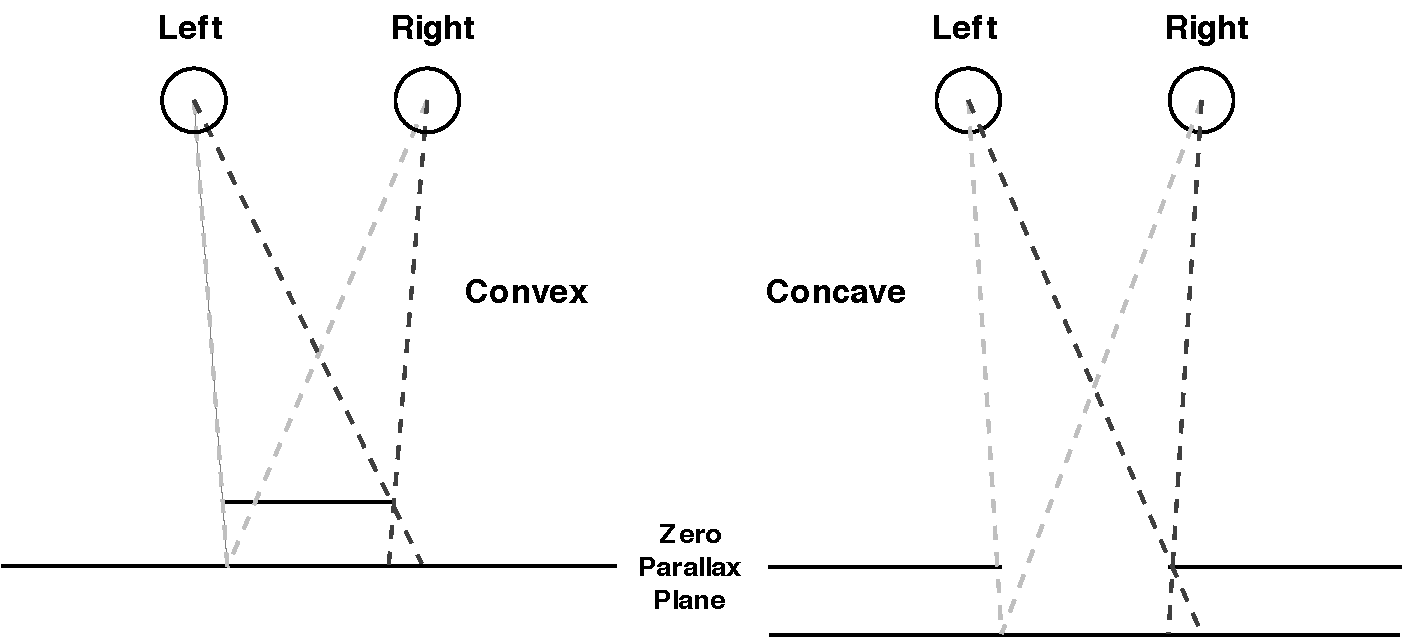
\includegraphics[width=15.5cm]{media/rds.pdf}
\caption{RDS of Convex and Concave surfaces can be created in different ways\label{ccRDS}}
\end{center}
\end{figure*}

\paragraph{}
The second algorithm is split into two parts, which deal with convex and concave stereograms separately.
This deals with subtle problems with partial occlusion (see figure \ref{ccRDS}).
It also uses different patterns for fore- and background.
Using pre-calculated patterns was loosely inspired by a paper from Gonzalez and Krause\cite{GenRDS}, which allowed different densities for object and background.

Using different colors for the foreground and the background makes the object defined in the depth map stand out. This helps visibility, but that way the shape of the object itself can not be used to validate fusion. Depending on the offset of fore- and background and the size of the random dot stereogram, it is not easily monocularly visible if the shape is convex or concave.

Both methods are simplified, the virtual cameras are always at the same relative position of the pixel in the depth map that is processed, similar to a parallel projection.

\paragraph{Convex}
The algorithm for convex shapes treats the depth map as a source to calculate the new position of pixel in a source pattern.
The calculated offset is used to displace the surface into the destination image.
The shape is shifted horizontally and appears to come out of the surface.
This is equivalent to tracking the surface of the object, and projecting the observed value onto the background (figure \ref{ccRDS}, left).
The same effect can be achieved by tracking the background, but in border cases one eye would see the background, while the other eye sees the foreground.

\paragraph{Concave}
The algorithm for concave shapes works slightly different.
It treats the depth map as a source to calculate the position of the pixel in a source pattern to place in the destination pattern.
The shape is not shifted, but its texture is.
It appears to go into the surface.
This is equivalent to tracking the background plane, and projecting the corresponding object pattern values onto the background (figure \ref{ccRDS}, right).
It can be achieved by tracking the object, but in border cases,  a point might come from the foreground for one eye, and the background for the other.

\subsubsection{Pattern stereogram}
\paragraph{}
Pattern stereograms are created similarly to random dot stereograms.
Instead of a random data source, they use a pre-computed pattern as foreground and background image.
This makes the shape stand out more and allows a high customizability of the pattern.
Possible sources include randomly generated noise images, photographed textures and randomly distributed shapes.


\section{Meshes}
\paragraph{}
An important requirement for the tool is, that it has to be able to display a wide range of stimuli. Not only the depth cues (see section \ref{Cues}) have to be individually controllable, also the possible shapes of objects have to span a wide range.

The tool supports only few basic object types, such as Pixel Planes (raster image data), parallelograms, and parallelepipeds. Implementing every desired type in code is neither feasible nor desirable.
Instead, the same approach as with textures is taken: An external tool that is familiar to the user is used to create a shape, and this shape is then loaded and displayed by the tool. By far the most commonly used method to store models is \textit{Mesh}. A mesh is a surface defined by points, which are connected by edges, to form faces. Other methods include \textit{NURBS}, \textit{Constructive Solid Geometry} and many types of \textit{Parametric Surfaces}. They are less popular, and often harder to handle than meshes.

There are a number of possibilities to implement this design. A mesh library can be used to load, render and modify meshes in an easy way. A scene graph library provides not only mesh support, but also the handling of whole scene hierarchies. Mesh importer libraries make it easier to parse models into a custom data format.


\subsection{Mesh Libraries}
\paragraph{}
Mesh libraries provide an API for loading, manipulating and rendering meshes. \textit{OpenMesh} is a very powerful library with a half-edge data structure. It offers a wide array of possibilities to customize storage, access and manipulation. It does not handle rendering.

\paragraph{}


\subsection{Mesh Formats}
\paragraph{}

\subsection{Mesh Creation}
\paragraph{}


\end{multicols}

\newpage

\begin{multicols}{2}

\tableofcontents

\end{multicols}

\appendix

\begin{thebibliography}{12}
\bibitem{AntRDS}
Bergua A., Skrandiesb W., 2000,
\textit{An early antecedent to modern random dot stereograms - 'The Secret Stereoscopic Writing' of Ram\'on y Cajal}.
Int. J. of Psychophysiology 36, 69-72\\
\url{http://dx.doi.org/10.1016/S0167-8760(99)00111-7}

\bibitem{BellRDS}
Julesz B., 1960.
\textit{Binocular depth perception of computer-generated patterns}.
Bell Syst. Tech. J. 39, 1125-1162.\\
\url{http://doi.apa.org/?uid=1961-01385-001}

\bibitem{GenRDS}
Gonzalez F., Krause F., 1994.
\textit{Generation of dynamic random-element stereograms in real time with a system based on a personal computer}.
Med. \& Biol. Eng. \& Comput., 1994, 32, 373-376.\\
\url{http://dx.doi.org/10.1007/BF02524687}

\bibitem{DepthCues}
Cutting J., Vishton P., 1995.
\textit{Perceiving layout and knowing distances: The integration, relative potency, and contextual use of different information about depth}.
In W. Epstein \& S. Rogers (Eds.), Handbook of perception and cognition, Vol. 5, 69-117. San Diego, CA: Academic Press.\\
\url{http://dx.doi.org/10.1016/B978-012240530-3/50005-5}

\end{thebibliography}

% Might only work in KOMA script (scrarticle)
\renewcommand*\refname{Links}

\begin{thebibliography}{12}
\bibitem[a]{proj} \url{http://en.wikipedia.org/wiki/Graphical_projection}
\bibitem[b]{parallel} \url{http://en.wikipedia.org/wiki/Parallel_projection}
\bibitem[c]{perspective} \url{http://en.wikipedia.org/wiki/Perspective_projection}
\bibitem[d]{painters} \url{http://en.wikipedia.org/wiki/Painter's_algorithm}
\bibitem[e]{zbuffer} \url{http://en.wikipedia.org/wiki/Z-buffering}
\bibitem[f]{fog} \url{http://www.opengl.org/documentation/specs/version1.1/glspec1.1/node90.html}
\bibitem[g]{accommodation} \url{http://en.wikipedia.org/wiki/Accommodation_(eye)}
\bibitem[h]{triangulation} \url{http://en.wikipedia.org/wiki/Triangulation}
\bibitem[i]{scenegraph} \url{http://www.realityprime.com/articles/scenegraphs-past-present-and-future}
\bibitem[j]{turing} \url{http://en.wikipedia.org/wiki/Turing_completeness}
\bibitem[k]{procedural} \url{http://en.wikipedia.org/wiki/Procedural_programming}
\end{thebibliography}




\end{document}
\end
